\chapter{VIRTUAL MOUSE USING HAND GESTURE PYTHON}

Mouse adalah salah satu penemuan yang luar biasa pada dunia tekhnologi Human-computer Interaction (HCI), saat ini mouse nirkabel atau mouse bluetooth masih menggunakan perangkat keras karena membutuhkan batrai dan kabel 	untuk menghubungkan nya ke pc. Dalam sistem virtual mouse yang diusulkan, keterbatasan ini dapat diatasi dengan menggunakan webcam atau kamera built-in untuk menangkap gerakan tangan dan mendeteksi ujung jari menggunakan visi komputer, algoritma yang digunakan dalam sistem ini menggunakan algoritma mechine learning berdasarkan gerakan tangan yang telah terdeteksi, komputer dapat dikontrol secara virtual dan dapat melakukan fungsi klik kanan, klik kiri, drag and drop, scrolling dan fungsi mouse lainya tanpa membutuhkan perangkat keras.


\section{Virtual Mouse Hand Gesture}

\begin{enumerate}
  \item \textbf{Artificial Intelegence} \\
    Artificial Intelegence (AI) adalah cabang ilmu komputer yang mensimulasikan kecerdasan yang dimiliki oleh manusia yang diimplementasikan kedalam suatu program komputer, kecerdasan buatan adalah aktivitas mesin yang menampilkan prilaku yang dianggap hampir menyerupai kecerdasan yang dimiliki oleh manusia, sehingga bisa dikatakan AI merupakan sistem atau program kompute yang mampu melakukan pekerjaan dan memutuskan sesuatu seperti layaknya manusia.
    AI juga merupakan tekhnologi yang memungkinkan mesin bisa mengerti apa yang pengguna inginkan dan butuhkan, misalnya untuk menciptakan mesin yang dapat menidentifikas suara dan mampu memberikan \textit{return} atau timbal balik dari mesin tersebut. 
  \item \textbf{Machine Learning}  \\
    Istiah \textit{mechine learning}  pertama kali dikemukakan oleh beberapa ilmuan matematika seperti Adren Marie Lagandrie, Thomas Bayes dan Andrey Mrkov pada tahun 1920-an dengan mengemukakan dasar-dasar \textit{mechine learning} dan konsepnya. sejak saat itu ML banyak yang mengembangkan. salah satu contoh dari penerapan ML yang cukup terkenal adalah \textit{deep blue} yang dibuat oleh IBM pada tahun 1996.
    Teknologi \textit{mechine learning}  adalah mesin yang dikembangkan untuk bisa belajar dengan sendirinya tanpa arahan dari pengguna atau \textit{user}, pembeljaran \textit{mechine learning}  dikembangkan berdasarkan disiplin ilmu lainya seperti statistika, matematika dan data mining sehingga mesin dapat belajar dengan menganalisis data tanpa perlu di program ulang atau diperintah.
    untuk bisa mengoprasikan \textit{mechine learning} secara optimal terdapat 3 metode yaitu: 
    \begin{figure} [ht] \centering
      % Nama dari file gambar yang diinputkan
      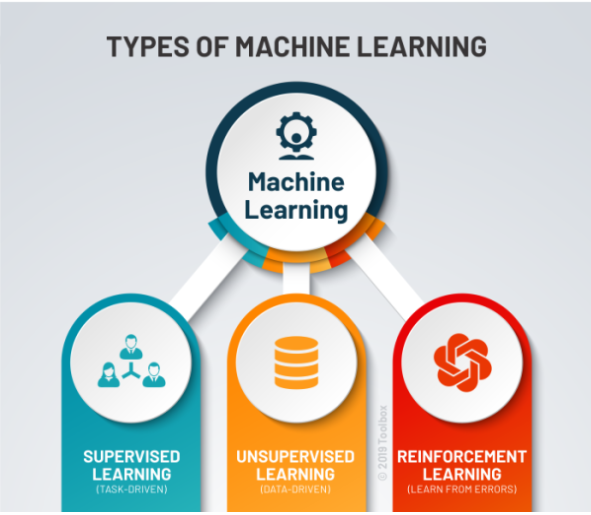
\includegraphics[scale=0.9]{gambar/metode_ML.png}
      % Keterangan gambar yang diinputkan
      \caption{tiga metode atau tipe mechine learning (Sumber: ekrut.com)}
      % Label referensi dari gambar yang diinputkan
      \label{fig:OrganizationStructure}
    \end{figure}
    \begin{enumerate}[nolistsep]
      \item \textit{\textbf{Supervised Learning}}\\
        Metode supervised learning dilakukan dengan pemberian label pada dataset  yang digunakan oleh machine learning dan diklasifikasikan oleh pengembang dengan memungkinkan algoritma melihat tingkat akurasi kinerjanya. Pengawasan machine learning dalam metode ini dilakukan oleh data berlabel yang nantinya membuat machine learning mempelajari apa hubungan dan ketergantungan antar data.
        Cara kerja metode ini adalah memasukkan informasi sebagai input dan data berlabel sebagai hasil atau output. Input dalam machine learning pinjaman bank misalnya dapat berupa data rinci seperti usia, gaji, jumlah pinjaman, jumlah terutan, riwayat pinjaman, dan lain sebagainya. Sedangkan output-nya dapat berupa hasil dari keseluruhan jumlah orang yang membayar pinjaman dan berapa jumlah orang gagal membayar.
      \item \textit{\textbf{Semi-supervised Learning (Unsupervised)}} \\
        Metode \textit{semi-supervised learning} bisa disebut juga sebagai metode \textit{machine learning} tanpa pengawasan. Sehingga, prosesnya dilakukan pada dataset mentah yang tidak berlabel dan algoritma \textit{machine learning} akan mencoba mengidentifikasi pola dan relasi antar data tanpa bantuan dari pengembang.
        Metode \textit{unsupervised learning} pada umumnya memang tidak ada bantuan dari manusia agar komputer benar-benar mempelajari sebuah data dan relasinya secara mandiri. Dalam kasusnya, dataset tidak berlabel dan mesin secara komputasi akan mengidentifikasi pola dalam data. \textit{Unsupervised learning} digunakan untuk memudahkan pengembang mengambil keputusan.
        Dalam kasus \textit{mechine learning} pinjaman bank tadi, sebuah \textit{unsupervised learning} dapat mendeteksi anomali atau mengungkap transaksi atau pembayaran yang curang. \textit{Unsupervised learning}  dapat secara otomatis mencari informasi setelah mengelompokkan pola dari semua data peminjam dari sebuah bank dan memunculkannya sebagai sebuah output tanpa harus memasukkan data berlabel secara rinci.
      \item \textit{\textbf{Reinforcement Learning}} \\
        Metode \textit{machine learning} yang satu ini dijalankan dengan menggunakan dataset bersistem “rewards/punishment” dan menawarkan umpan balik ke algoritma untuk belajar dari pengalamannya secara coba-coba (random). Metode “coba-coba” ini hampir sama dengan sistem pemahaman pola yang dilakukan manusia yaitu belajar dari percobaan.

        Hal ini yang lantas membuat metode ini disebut sebagai \textit{machine learning} dengan tipe penguatan pembelajaran. Algoritma dalam metode ini akan belajar secara terus-menerus dari lingkungan atau kebiasaan interaksi yang berhubungannya dengannya. Dari sana nantinya algoritma akan mendapat “rewards” atau “punishment” sebagai impresi positif dan negatif berdasarkan tindakan percobaannya.
      
        Dalam kasus machine learning pinjaman bank, algoritma reinforcement learning akan mengklasifikasikan pelanggan berisiko tinggi secara default dan akan mengelompokkan pelanggan yang gagal bayar sebagai aspek negatif secara otomatis.  
    \end{enumerate}
  \item \textbf{Deep Learning} \\ 
    Deep learning adalah salah satu subbidang dari \textit{mechine learning} yang algoritmanya terinpirasi dari otak manusia. Saat ini teknik \textit{deep learning} telah diterapkan diberbagai bidang teknologi seperti \textit{self-driving car}, \textit{deep learning} yang disusun berdasarkan arsitektur otak manusia dinamakan \textit{Artificial Neural Network} atau ANN. ia mampu belajar dan beradaptasi teradap sejumlh besar data serta menyelesaikan berbagai permasalahan yang sulit diselesaikan dengan algortma \textit{mechine learning} lainnya. 
    \begin{enumerate}[nolistsep]
      \item \textbf{\textit{Convolutional Neural Network (CNN)}}\\
        CNN terdiri dari banyak layer untuk memproses dan mengekstrak fitur dari data. Ia biasanya digunakan untuk memproses gambar dan mendeteksi objek. Saat ini, CNN banyak digunakan untuk mengidentifikasi citra satelit, citra medis, dan mendeteksi anomali.
      \item \textbf{\textit{Recurrent Neural Network (RNN)}}\\
        \textit{Recurrent Neural Networks (RNN)} merupakan salah satu bentuk arsitektur \textit{Artificial Neural Networks (ANN)} yang dirancang khusus untuk memproses data yang bersambung/ berurutan (sequential data). RNN biasanya digunakan untuk menyelesaikan permasalahan data historis atau time series, contohnya data ramalan cuaca. Selain itu, RNN juga dapat diimplementasikan pada bidang natural language understanding (pemahaman bahasa alami), misalnya  translasi bahasa.
      \item \textbf{\textit{{Long Short Term Memory Network (LTSM)}}}
    \end{enumerate}
  
\end{enumerate}

\section{}

Masalah yang akan \lipsum[3][1-2] adalah:

\begin{enumerate}[nolistsep]

  \item Bagaimana cara \lipsum[3][3-5]

  \item \lipsum[3][6-8]

\end{enumerate}

\section{Tujuan}

Tujuan dari \lipsum[4][1-3] adalah:

\begin{enumerate}[nolistsep]

  \item Membuat \lipsum[4][4-5]

  \item \lipsum[4][6-9]

\end{enumerate}

\section{Manfaat}

Manfaat dari \lipsum[5][1-3] adalah:

\begin{enumerate}[nolistsep]

  \item Mempermudah \lipsum[5][4-5]

  \item \lipsum[5][6-10]

\end{enumerate}

\section{Waktu dan Tempat Pelaksanaan}

Kerja praktik akan dilaksanakan pada \lipsum[6][1-3]

\section{Metodologi Kerja Praktik}

Metode yang \lipsum[7][1-5] yaitu:

\begin{enumerate}[nolistsep]

  \item \textbf{Perumusan Masalah}

  Pada tahap ini \lipsum[7][6-9]

  \item \textbf{Studi Literatur}

  Pada tahap ini \lipsum[7][10-13]

  \item \textbf{Analisis dan Perancangan Sistem}

  Pada tahap ini \lipsum[8][1-2]

  \item \textbf{Implementasi Sistem}

  Pada tahap ini \lipsum[8][3-6]

  \item \textbf{Pengujian dan Evaluasi}

  Pada tahap ini \lipsum[8][7-12]

\end{enumerate}

\section{Sistematika Penulisan}

Laporan kerja praktik akan terbagi menjadi \lipsum[9][1] yaitu:

\begin{enumerate}[nolistsep]

  \item \textbf{Bab I Pendahuluan}

  Bab ini berisi \lipsum[9][2-4]

  \item \textbf{Bab II Profil Perusahaan}

  Bab ini berisi \lipsum[9][5-7]

  \item \textbf{Bab III Tinjauan Pustaka}

  Bab ini berisi \lipsum[9][8]

  \item \textbf{Bab IV Desain dan Implementasi}

  Bab ini berisi \lipsum[10][1-2]

  \item \textbf{Bab V Pengujian dan Evaluasi}

  Bab ini berisi \lipsum[10][3-4]

  \item \textbf{Bab VI Kesimpulan dan Saran}

  Bab ini berisi \lipsum[10][5-8]

\end{enumerate}
